% Settings {{{
\documentclass[t, 11pt, xcolor=dvipsnames]{beamer}
\usepackage{textcomp}
\usepackage{mathtools}
\usepackage{pdfpages}
\usepackage{graphicx}
\usepackage{tikz}
\usepackage{multimedia}
\usepackage{transparent}
\usepackage{textpos}
\usetikzlibrary{calc}
\usepackage{amsmath}

% Fonts
\usefonttheme{professionalfonts} % using non standard fonts for beamer
%\usefonttheme{serif} % default family is serif

%%%%%%%%%%%%%%%%%%%%%%%%%%%%%%%%%%%%%%%%%%%%%%%%%%%%%%%%%%%%

\usetheme{Berlin}

\definecolor{CLICbg}{rgb}{0.113, 0.125, 0.129}
\definecolor{CLICfg}{rgb}{0.895, 0.895, 0.895}

\setbeamercolor{structure}{fg=CLICbg} % itemize, enumerate, etc
\setbeamercolor{structure}{bg=CLICbg} % itemize, enumerate, etc
\setbeamercolor{section in toc}{fg=CLICbg} % TOC sections

\addtobeamertemplate{frametitle}{}}}
% Opening details {{{
\subtitle{PH40024 Contemporary Physics}
\title{Emergent Collective Dynamics of Skyrmions}
\author{ Insert image } %\includegraphics[width=0.65\textwidth]{title.jpg}}
\titlegraphic{\vspace{-4em}\begin{flushright}Donovan Webb\end{flushright}}
\date{}

\AtBeginSection[]{
  \begin{frame}
  \vfill
  \centering
  \begin{beamercolorbox}[sep=8pt,center,shadow=false,rounded=false]{title}
    \usebeamerfont{title}\insertsectionhead\par%
  \end{beamercolorbox}
  \vfill
  \end{frame}
}


\begin{document}

\setbeamertemplate{navigation symbols}{}
\begin{frame}[plain]
\setbeamercolor{title}{bg=white,fg=CLICbg}
  \maketitle
\setbeamercolor{title}{bg=CLICbg,fg=CLICfg}
\end{frame}
\addtocounter{framenumber}{-1} % Don't count title slide

%}}}
% Slides {{{
% 15 minute presentation 14:20 Friday 19/11/21 3WN 3.8. Aiming for 5-7 slides only!
\begin{frame}[plain]{Outline}
  \small
  \begin{itemize}
    \item Motivation. Why is this interesting! \\
      {\tiny new dynamic materials.}
    \item Overall overview \\
    \begin{enumerate}
        \tiny
        \item Will discuss what skyrmions are.  \\
        \item Why they are particle like and can be active matter. \\
        \item They're emergent dynamic behaviour --- collective movement and clustering. \\
        \item Finish with applications \\
            \end{enumerate}
    \item Physics and arrangement of skyrmion \\
    \item pair movement \\
    \item large group movement \\
    \item Uses of technology \\
    \item Repeat overview \\
  \end{itemize}
  \hypertarget<1>{slide1}{}
\end{frame}

\begin{frame}[plain]{intro}
  Starting with the end results/applications/motivation \\
  ref 33-36\\
  Movie \\
\end{frame}

\begin{frame}[plain]{intro}
  Active soft matter \\
  complex dynamics \\
  Topological 2D solitons --- skyrmions act like particles \\
  exhibit collective motion --- In random directions! \\
  Observe complex clustering behaviour \\
  Out of equilibrium elastic interactions \\
  \hypertarget<1>{slide2}{}
\end{frame}

\begin{frame}[plain]{Skyrmions}
  Physical reliazation in chiral LC \\
  \begin{center}
    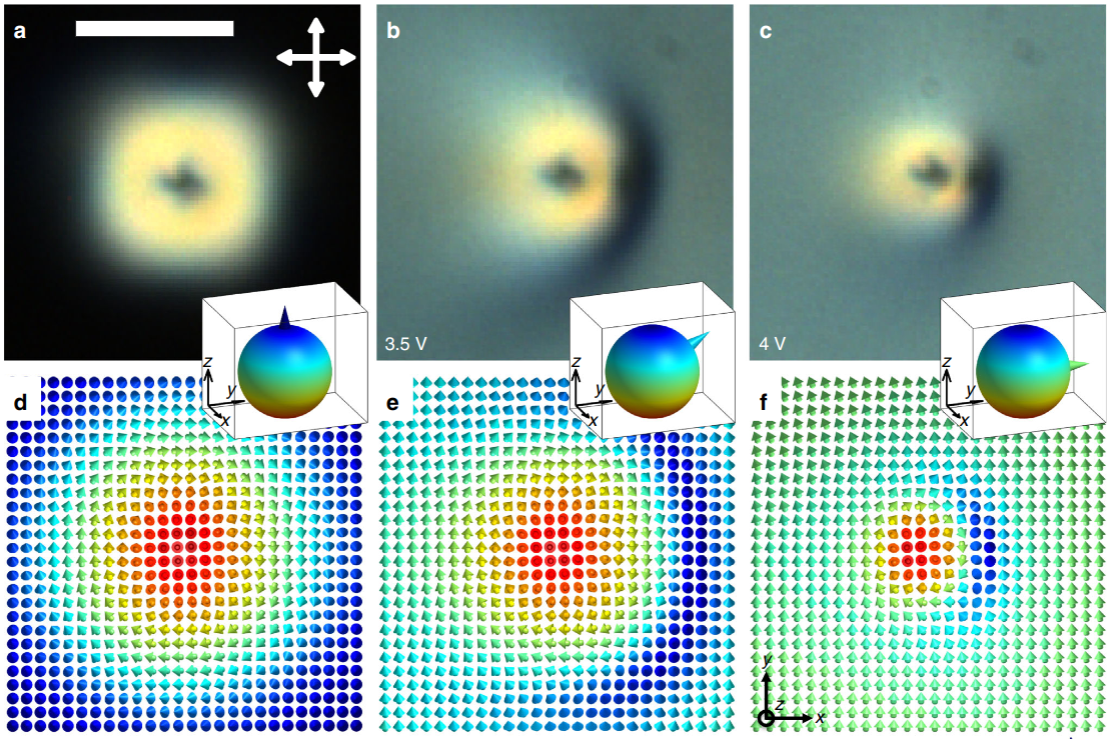
\includegraphics[width=0.35\textwidth]{images/skyrm.png}
    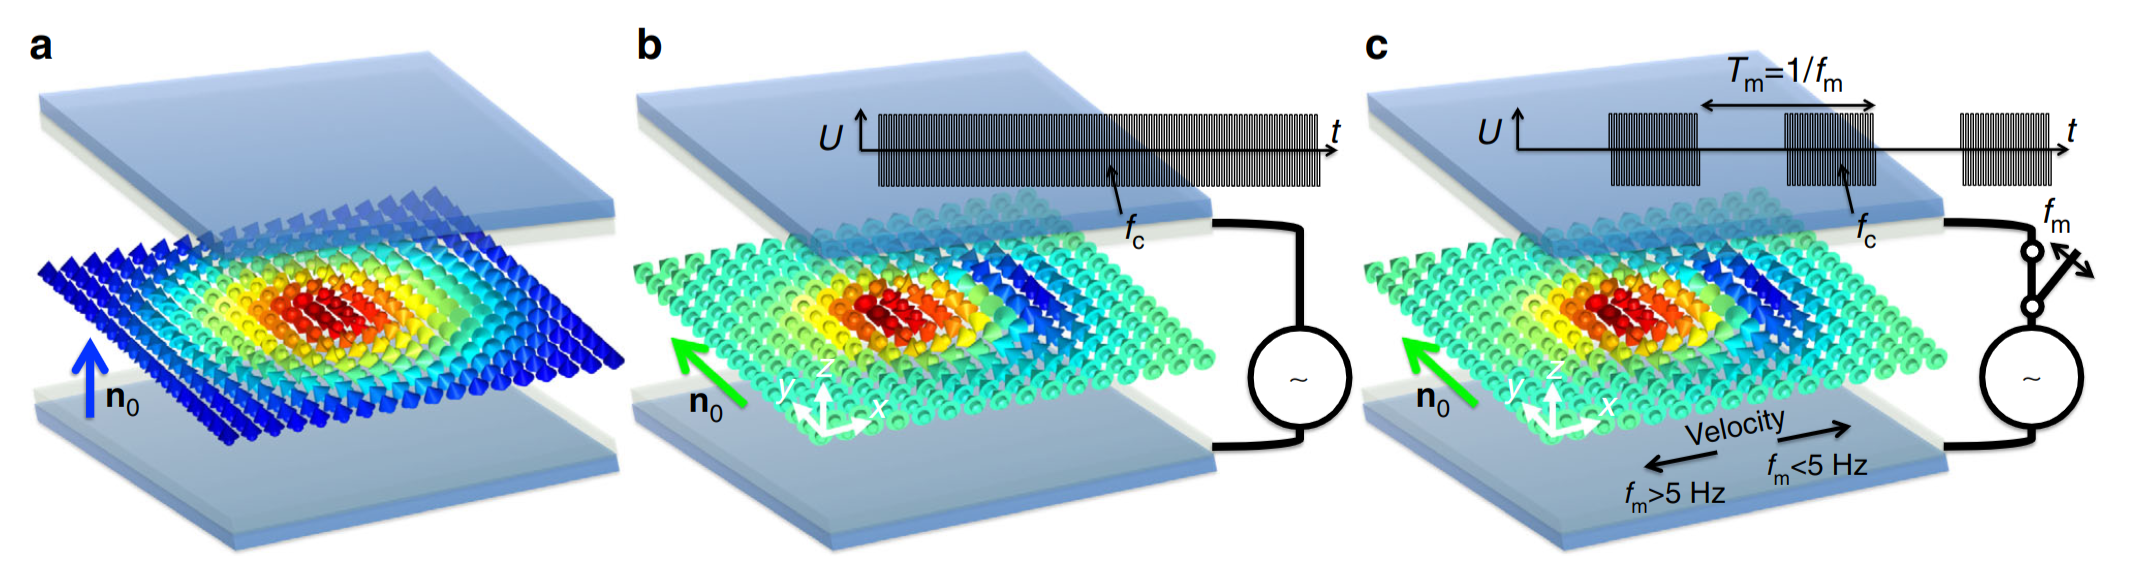
\includegraphics[width=0.35\textwidth]{images/plate.png}
    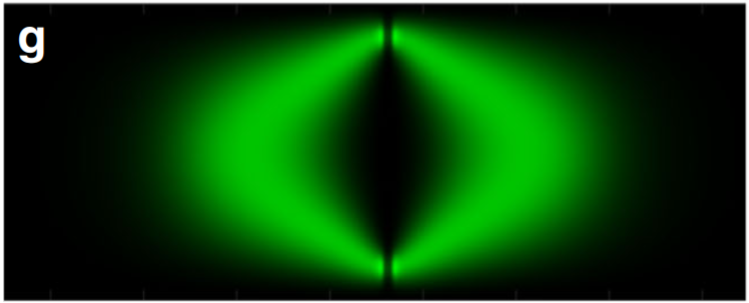
\includegraphics[width=0.35\textwidth]{images/cross_sec.png}
  \end{center}
\end{frame}

\begin{frame}[plain]{Squirming Skyrmions}
  Movement \\
    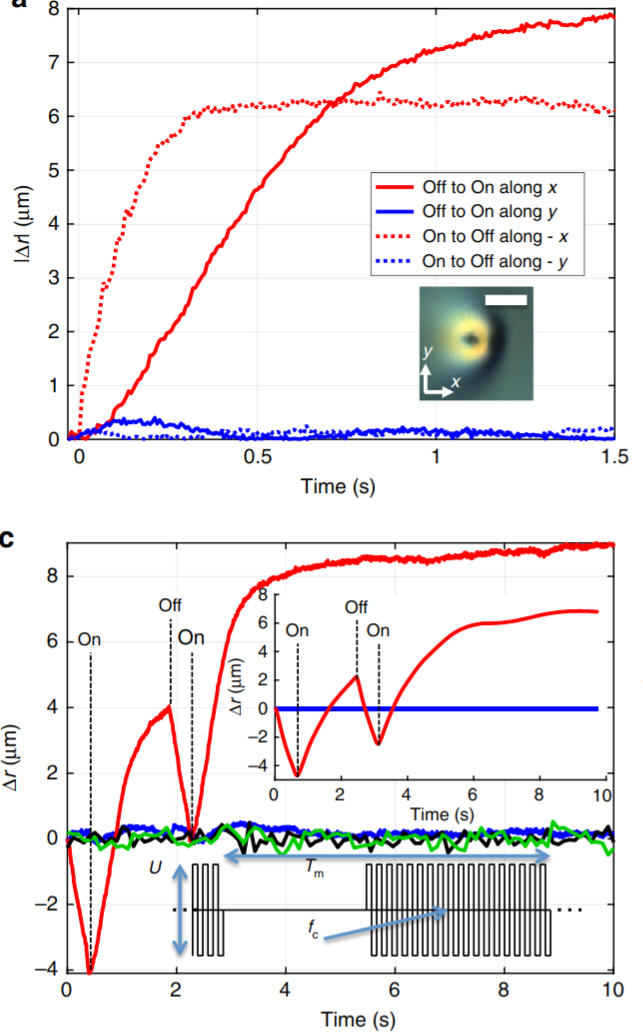
\includegraphics[width=0.35\textwidth]{images/squirm.png}
    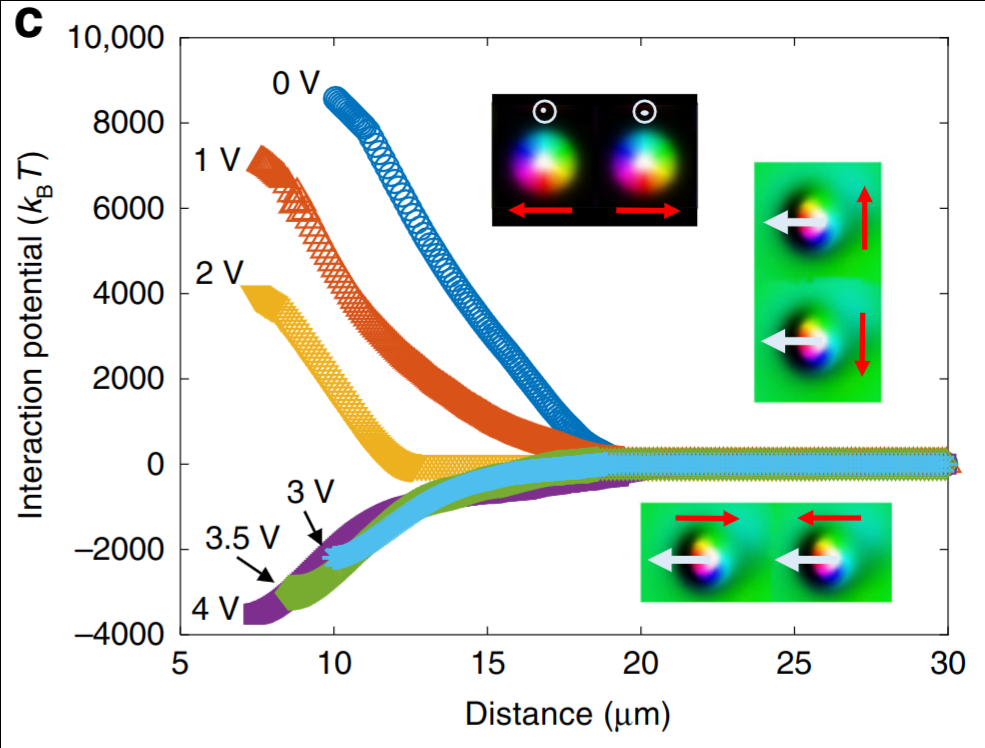
\includegraphics[width=0.35\textwidth]{images/2part.png}
  Two particle interactions \\
\end{frame}

\begin{frame}[plain]{Skyrmions}
  Many particle elastic interactions \\
  Coherent motion \\
    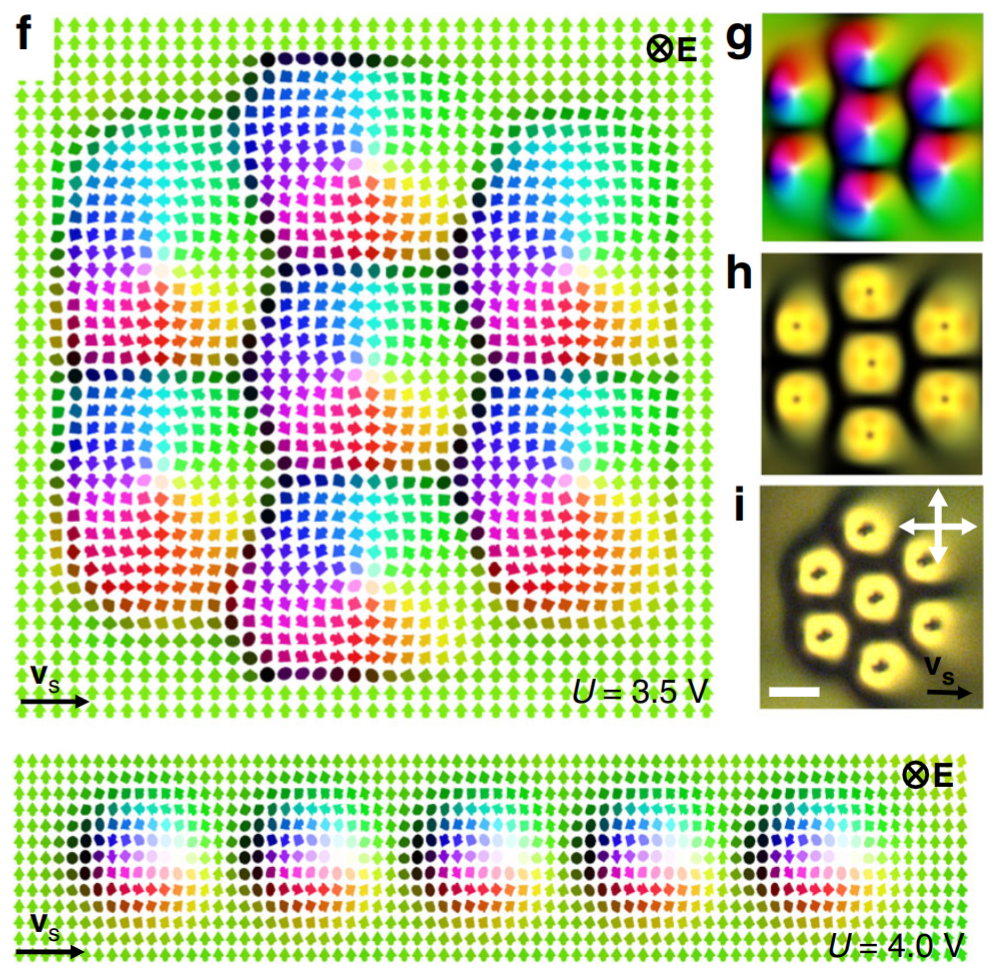
\includegraphics[width=0.35\textwidth]{images/cluster.png}
    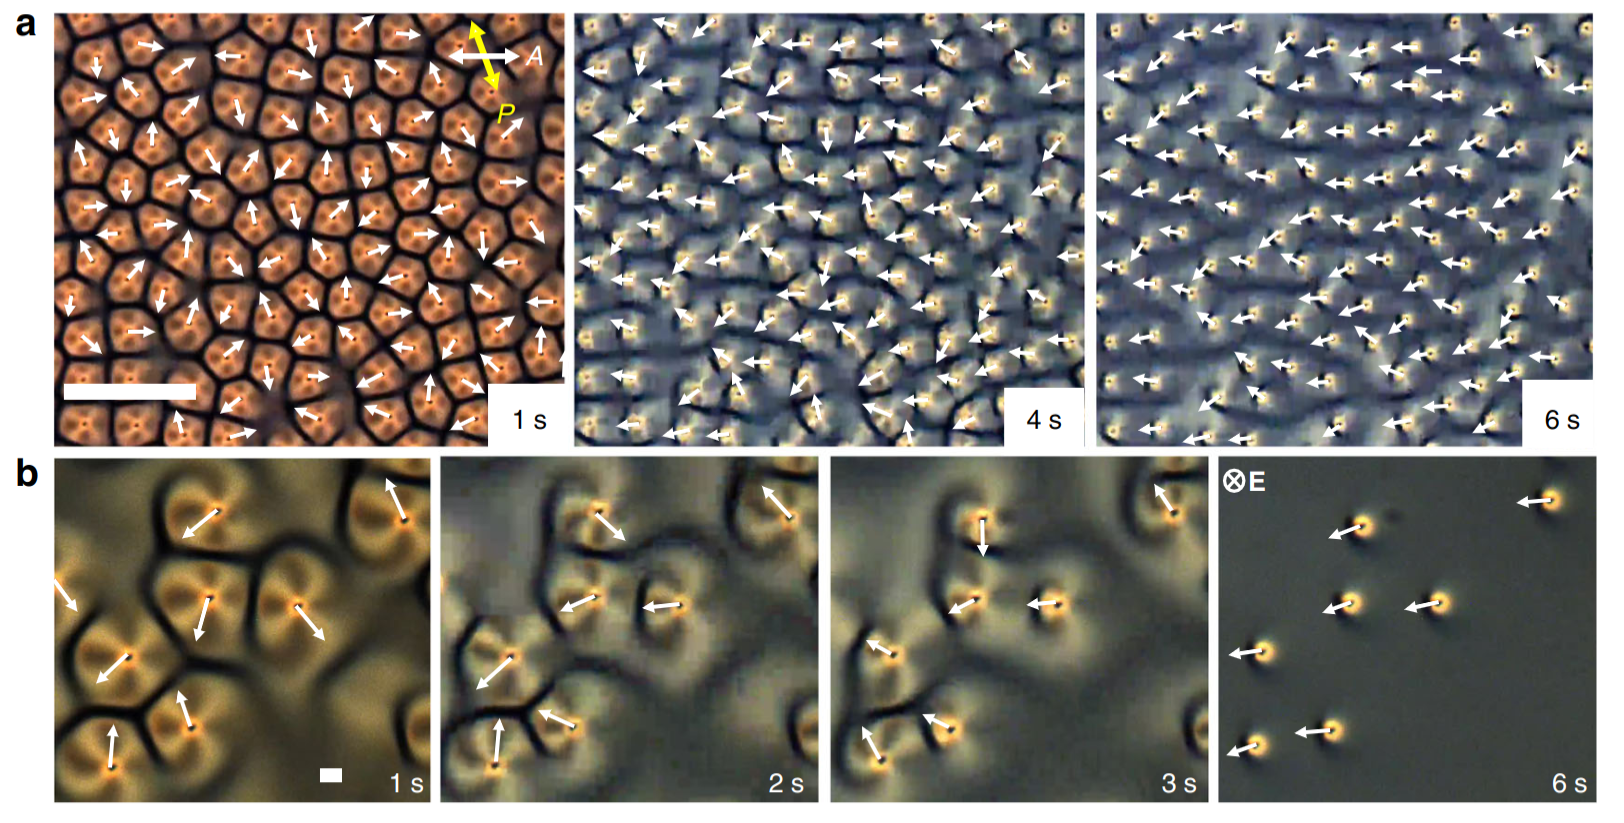
\includegraphics[width=0.35\textwidth]{images/manypart.png}
    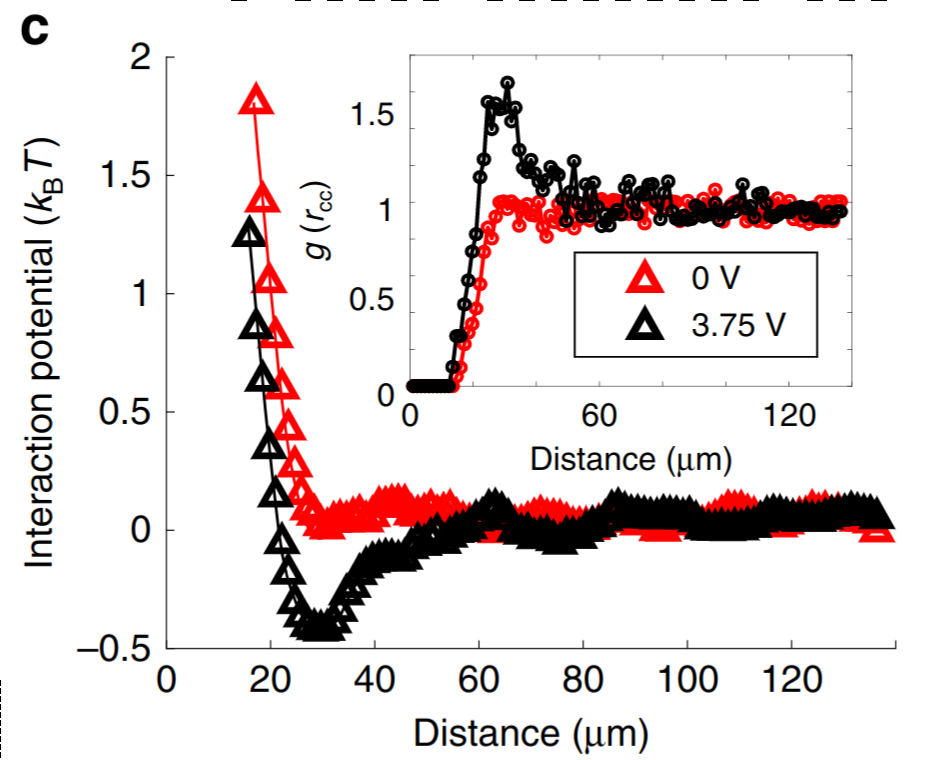
\includegraphics[width=0.35\textwidth]{images/LJ.png}
  \hypertarget<1>{slide3}{}
\end{frame}

\begin{frame}[plain]{Skyrmions}
  Varying oscillation and field \\
    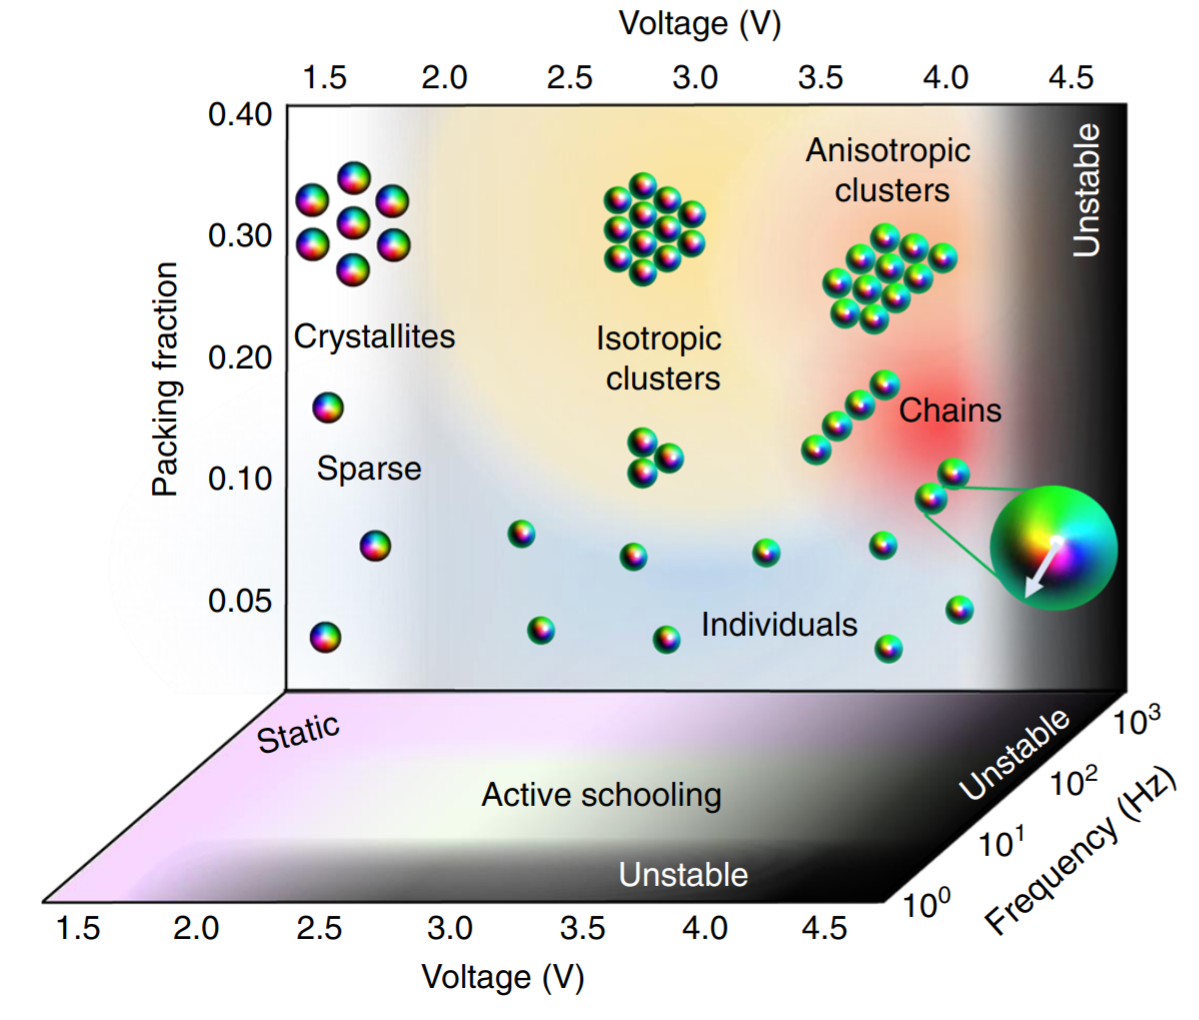
\includegraphics[width=0.35\textwidth]{images/phase.png}
\end{frame}

\begin{frame}[plain]{Conclusions}
  Applications \\
\end{frame}

\begin{frame}[plain]{Conclusions}
  Reiteration \\
  (and references) \\
\end{frame}
%}}}
% References {{{
\begin{frame}[plain]{References}
  \scriptsize
  \begin{enumerate}
  \item  M. M. Smith, V. A. Warren, B. S. Thomas, R. M. Brochu, E. A. Ertel, S. Rohrer, J. Schaeffer, D. Schmatz, B. R. Petuch, Y. S. Tang, P. T. Meinke, G. J. Kaczorowski, and C. J. Cohen, Biochemistry, 2000, 39, 5543-5554 \\
  \item J. G. Ondeyka, G. L. Helms, O. D. Hensens, M. A. Goetz, D. L. Zink, A. Tsipouras, W. L. Shoop, L. Slayton, A. W. Dombrowski, J. D. Polishook, D. A. Ostlind, N. N. Tsou, R. G. Ball, and S. B. Singh, J. Am. Chem. Soc. 1997, 119, 8809-8816 \\
  \item R. Tanifuji, A. Minami, H. Oguri and H. Oikawa, Nat. Prod. Rep. 2020, 37, 1098 \\
  \item K. C. Van de Bittner, M. J. Nicholson, L. Y. Bustamante, S. A. Kessans, A. Ram, C. J. van Dolleweerd, B. Scott, and E. J. Parker, J. Am. Chem. Soc. 2018, 140, 582-585 \\
  \item A. B. Smith III, A. H. Davulcu, Y. S. Cho, K. Ohmoto, L. Kuerti, and H. Ishiyama, J. Org. Chem. 2007, 72, 4596-4610 \\
  \item A. B. Smith III, L. Kuerti, A. H. Davulcu, Y. S. Cho, and K. Ohmoto, J. Org. Chem. 2007, 72, 4611-4620 \\
  \item Y. Zou, X. Li, Y. Yang, S. Berritt, J. Melvin, S. Gonzales, M. Spafford, and A. B. Smith III, J. Am. Chem. Soc. 2018, 140, 9502-9511 \\
  \item ACS. Cent. Sci. 2018 PMID: 30648156 \\
  \end{enumerate}
\end{frame}
%}}}
\end{document}
